% template adapted from https://github.com/jgm/pandoc-templates/blob/master/default.latex
%%%%%%%%%%%%%%%%%%%%%%%%%%%%%%%%%%%%%%%%%%%%%%%%%%%%%%%%%%%%%%%%%%%%%%%%%%%%%%%%%%%%%%%%%

% Options for packages loaded elsewhere
\PassOptionsToPackage{unicode=true}{hyperref}
\PassOptionsToPackage{hyphens}{url}
  \PassOptionsToPackage{dvipsnames,svgnames*,x11names*}{xcolor}


\documentclass[
  11pt,
  french,
  A4paper,
  extrafontsizes,onecolumn,openright
  ]{memoir}

% Font family: lmodern by default
  \usepackage{lmodern}

% Double (or whatever) spacing

\usepackage{amssymb, amsmath}
\usepackage{ifxetex,ifluatex}
\usepackage{fixltx2e} % provides \textsubscript

% mathspec: arbitrary math fonts
  \usepackage{unicode-math}
\defaultfontfeatures{Ligatures=TeX,Scale=MatchLowercase}

% More font families
% Main font
% Specific sanserif font
% Specific monotype font
% Specific math font
% Chinese, Japanese, Corean fonts

% Use upquote if available, for straight quotes in verbatim environments
\IfFileExists{upquote.sty}{\usepackage{upquote}}{}
% Use microtype if available
\IfFileExists{microtype.sty}{%
\usepackage[]{microtype}
\UseMicrotypeSet[protrusion]{basicmath} % disable protrusion for tt fonts
}{}

% Verbatim in note

\usepackage{xcolor}

\usepackage{hyperref}
\hypersetup{
            pdftitle={Trajectoires de biodiversité en forêt tropicale exploitée},
            pdfauthor={Ariane Mirabel},
            pdfkeywords={Biodiversity, Neotropical forests, Perturbation, Communities Ecology, Dynamic trajectories, Resilience},
            colorlinks=true,
            linkcolor=Maroon,
            citecolor=Blue,
            urlcolor=Blue,
            breaklinks=true}

% Don't use monospace font for urls
\urlstyle{same}


% Geometry package

% Listings package



% Tables
  \usepackage{longtable,booktabs}
  % Fix footnotes in tables (requires footnote package)
  \IfFileExists{footnote.sty}{\usepackage{footnote}\makesavenoteenv{longtable}}{}

% Graphics
  \usepackage{graphicx,grffile}
  \graphicspath{{images/}}
  \makeatletter
  \def\maxwidth{\ifdim\Gin@nat@width>\linewidth\linewidth\else\Gin@nat@width\fi}
  \def\maxheight{\ifdim\Gin@nat@height>\textheight\textheight\else\Gin@nat@height\fi}
  \makeatother
  % Scale images if necessary, so that they will not overflow the page
  % margins by default, and it is still possible to overwrite the defaults
  % using explicit options in \includegraphics[width, height, ...]{}
  \setkeys{Gin}{width=\maxwidth,height=\maxheight,keepaspectratio}



\setlength{\emergencystretch}{3em}  % prevent overfull lines
\providecommand{\tightlist}{%
  \setlength{\itemsep}{0pt}\setlength{\parskip}{0pt}}

  \setcounter{secnumdepth}{5}

% set default figure placement to htbp
\makeatletter
\def\fps@figure{htbp}
\makeatother

% Include headers (preamble.tex) here
%%% Complete the preamble of the LaTeX template
%%%------------------------------------------------------------------------------

%%% PACKAGES 
\usepackage{lipsum} % Dummy text.

\usepackage{enumitem}

  % load polyglossia as late as possible as it *could* call bidi if RTL lang (e.g. Hebrew or Arabic)
  \usepackage{polyglossia}
  \setmainlanguage[]{french}
  \setotherlanguage[variant=american]{english}
  \setotherlanguage[variant=british]{english}
  \setotherlanguage[]{french}




\usepackage[style=authoryear-ibid,backend=bibtex,citestyle=verbose-inote,isbn=false,backref=true,giveninits=true,uniquename=init,maxcitenames=2,maxbibnames=150,sorting=nyt,sortcites=false]{biblatex}
\addbibresource{packages.bib}
\addbibresource{01ref-IntroG.bib}
\addbibresource{02ref-chap2Incert.bib}

% Specific commands for EcoFoG style. Must come after biblatex.
\usepackage{latex/BookTemplate}


% Title, author, etc. from YAML to LaTeX
%%%%%%%%%%%%%%%%%%%%%%%%%%%%%%%%%%%%%%%%%%%%%%%%%%%%%%%%%%

\title{Trajectoires de biodiversité en forêt tropicale exploitée}


\author{Ariane Mirabel}


\date{2018-07-18}


% Main title page with filigrane
%%%%%%%%%%%%%%%%%%%%%%%%%%%%%%%%%%%%%%%%%%%%%%%%%%%%%%%%%%

\newcommand{\MainTitlePage}[1][]{
	\SmallMargins % Margins
	\pagestyle{empty} % No header/footer
	~\\ % Print a character or the page will not exist
	\begin{textblock}{2}(30,10)
		\rule{1pt}{\paperheight-20mm}
	\end{textblock}
	\begin{textblock}{140}(50, 45)
		\flushright
		\begin{Spacing}{3}
			{\fontfamily{qtm}\selectfont\fontsize{45}{45}\selectfont \textsc{\thetitle}}
		\end{Spacing}
	\end{textblock}
	\begin{textblock}{140}(50, 125)
		\flushright
		{\fontfamily{qtm}\Large \theauthor}
	\end{textblock}
	\begin{textblock}{120}[1, 1](225, 297)
		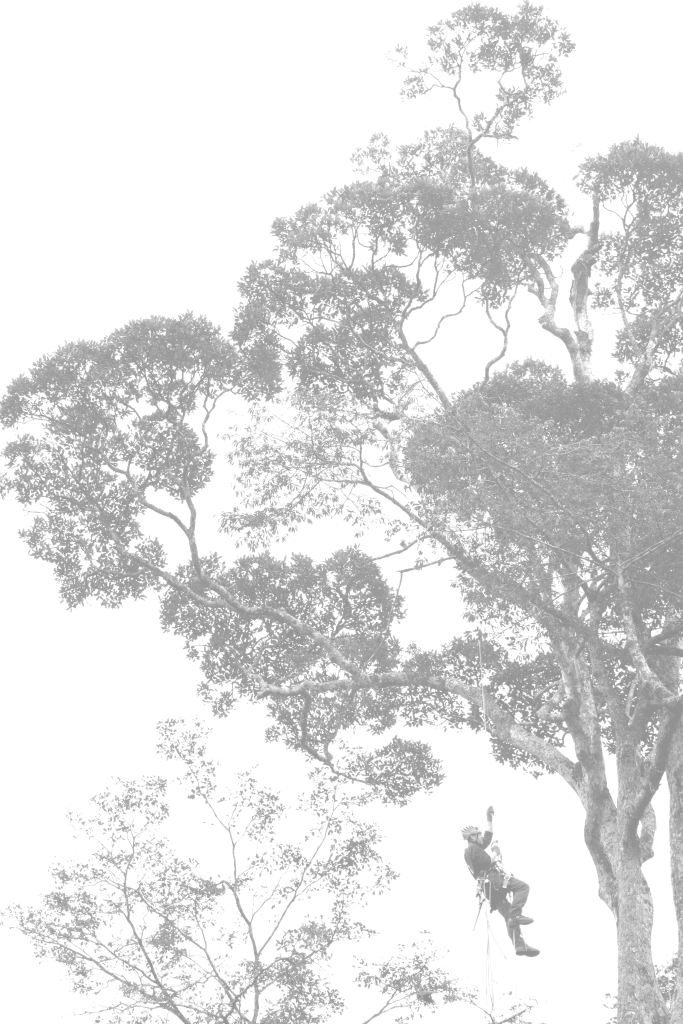
\includegraphics[width=10cm]{Filigrane}
	 \end{textblock}
	\begin{textblock}{140}[0, 1](50, 262)
		\normalfont	Version: \thedate
	\end{textblock}
	\newpage
	~\\ % Print a character or the page will not exist
	\begin{textblock}{140}(40, 40)
		#1
	\end{textblock}
	\begin{textblock}{140}[0,1](40, 270)
		\centering
    \includegraphics[width=5cm]{Logo-Lab}\\ \bigskip
		UMR \'Ecologie des forêts de Guyane\\
		\url{http://www.ecofog.gf}\\[3\baselineskip]
		Les opinions émises par les auteurs sont personnelles et n’engagent ni l’UMR EcoFoG ni ses tutelles.

    \tiny{Photographie en couverture: Hadrien Lalagüe}
	\end{textblock}
	\newpage
}

% PhD / HDR Thesis
%%%%%%%%%%%%%%%%%%%%%%%%%%%%%%%%%%%%%%%%%%%%%%%%%%%%%%%%%%

\usepackage[DocType=PhD, ED=UG, Ets=UG, DIS=ST]{latex/pdgUniv}

\specialty{Ecologie}
\defencedate{1er janvier 2018}
\lab{Ecologie des forets de Guyane}
% ==================
% Setup people like your boss, the jury team and the referees
% - First you need to define how number they will be in each category
%   It is done with the commands \nboss{n}, \nreferee{n} and \njudge{n}.
%   You can define more people in each category than the number given
%   but only the first "\npeople" will be print.
% - Then use the command \makesomeone{<category>}{<number>}{<name>}{<status>}{<other>}
%   where:
%     <category> should be select in ['boss', 'referee', 'judge']
%     <number>   is the rank for printing the person.
%                Only number <= "\npeople" will be printed
%     <name>     First name and las name of the people
%     <status>   Is (s)he a "charg\'e de recher" ou un "professeur d'universit\'e"...
%     <other>    What ever string you want to add (laboratory, jury member place...).
\njudge{7}
\makesomeone{judge}{1}{Prenom NomJury1}{Professeur d'Universite}{Membre du Jury}
\makesomeone{judge}{2}{Prenom NomJury2}{Professeur d'Universite}{Membre du Jury}
\makesomeone{judge}{3}{Prenom NomJury3}{Professeur d'Universite}{Membre du Jury}
\makesomeone{judge}{4}{Prenom NomJury4}{Professeur d'Universite}{Membre du Jury}
\makesomeone{judge}{5}{Prenom NomJury5}{Professeur d'Universite}{Membre du Jury}
\makesomeone{judge}{6}{Prenom NomJury6}{Professeur d'Universite}{Membre du Jury}
\makesomeone{judge}{7}{Prenom NomJury7}{Professeur d'Universite}{Membre du Jury}



% End of preamble
%%%%%%%%%%%%%%%%%%%%%%%%%%%%%%%%%%%%%%%%%%%%%%%%%%%%%%%%%%


\begin{document}
\frontmatter

% Title page
%%%%%%%%%%%%%%%%%%%%%%%%%%%%%%%%%%%%%%%%%%%%%%%%%%%%%%%%%%


\makeflyleaf
\newpage
~
\newpage




% Before Body
%%%%%%%%%%%%%%%%%%%%%%%%%%%%%%%%%%%%%%%%%%%%%%%%%%%%%%%%%%




% Contents
%%%%%%%%%%%%%%%%%%%%%%%%%%%%%%%%%%%%%%%%%%%%%%%%%%%%%%%%%%

\LargeMargins
{
\hypersetup{linkcolor=}
\setcounter{tocdepth}{3}
\tableofcontents
}


% Body
%%%%%%%%%%%%%%%%%%%%%%%%%%%%%%%%%%%%%%%%%%%%%%%%%%%%%%%%%%

\LargeMargins
\mainmatter

\chapter{Introduction générale}\label{introduction-generale}

Les forêts couvrent 30\% de la surface terrestre et assurent de nombreux
biens et services environnementaux, économiques et sociaux
indispensables à l'équilibre planétaire. Elles régulent le climat, la
qualité de l'eau, de l'air et des sols et abritent une diversité
biologique exceptionnelle. Elles subviennent aux besoins alimentaires de
la population mondiale et permettent son développement économique en
tant que source de matières premières, de revenus et d'opportunités de
développement. Enfin, indispensables au bien être des populations, elles
représentent des valeurs historiques, culturelles et patrimoniales
irremplaçables \autocites{FRA2015}{Tilman2014}. Malgré leur importance
les forêts sont aujourd'hui extrêmement menacées dans le contexte actuel
de changements globaux.

\section{Les forêts tropicales, au coeur des enjeux
actuels}\label{les-forets-tropicales-au-coeur-des-enjeux-actuels}

Par ``forêt'' ou ``ecosystème forestier'' on entend les assemblages de
plantes, animaux et microorganismes avec leur environnement qui
définissent une unité fonctionnelle, et dont les arbres sont les
composants essentiels \autocite{FRA2000}. Les forêts portent de forts
enjeux de conservation, en restant les régions les moins anthropisées et
en accueillant la diversité animale et végétale et les taux d'endémisme
les plus importants du globe \autocites{Myers2000}{Mittermeier2003}.

A l'échelle locale, les forêts entretiennent les cycles de l'eau et des
nutriments (azote, phosphore, etc), et régulent le climat et la
fertilité des sols \autocites{Malhi2008}{Isbell2017}. A l'échelle
globale, elles régulent les émission de gaz à effet de serre
(\emph{GES}) en compensant les émissions en tant que puits de carbone de
1.1 ± 0.8 PgC.yr\textsuperscript{--1}, mais sont également une source
potentielle de GES lorsque'elles sont dégradées et libèrent le carbone
stocké dans leur biomasse \autocites{Pan2011}{Roy2017}.

Les forêts assurent directement la subsistance de 500 millions de
personnes en tant que source de nourriture (par la chasse et la collecte
de produits forestiers non ligneux comestibles), d'eau, de matériaux de
construction, et d'énergie (par l'utilisation du bois de chauffage et de
cuisson). Elles sont de plus indispensables au bien-être des populations
et possèdent d'importantes dimensions culturelle, spirituelle et
patrimoniale. Enfin, l'exploitation forestière correspond à de forts
enjeux économiques: elle représente \textasciitilde{} 1\% du PIB
mondial, une part importante de l'emploi et rsete l'une des principales
sources d'énergie \autocites{CBDdiversity2011}{FAO2014}.

Indispensables et irremplaçables, les forêts disparaissent ou sont
dégradées à une vitesse croissante: entre 2013 et 2015 par exemple leur
surface globale a diminué de 3\% \autocite{FAO2009}. Elles subissent de
fortes pressions anthropiques allant des changements d'usage des terres,
tels que le déboisement pour l'élevage ou l'agriculture, à
l'exploitation du bois légale ou illégale, à la chasse ou à
l'introduction d'espèces invasives. Elles subissent également les
changements climatiques globaux qui augmentent la fréquence des
événements extrêmes tels que les sécheresses, les incendies, ou les
inondations\ldots{} \autocite{Pachauri2014}.

Une prise de conscience globale de ces pressions diverses a été
entérinée par la conférence des nations unies sur l'environnement et le
développement à Rio en 1992. De nombreux engagements politiques de
surveillance, de conservation de la biodiversité et de préservation du
fonctionnement des forêts ont pris mais les menaces persistent ou
s'accroissent malgré tout
\autocites{Summit1992}{Schlaepfer2000}{Dirzo2003a}{Morales-Hidalgo2015}.

Dans ce contexte les forêts tropicales sont particulièrement menacées.
Les bassins forestiers tropicaux représentent 19.6 million de km² et
représentent des enjeux économiques et de préservation primordiaux au
niveau mondial \autocites{Dirzo2003a}{Hansen2013}. Ils accueillent la
diversité biologique la plus élevée au monde et sont les plus grandes
forêts n'ayant jamais connu de forte perturbation anthropique
\autocites{Gentry1988}{FAO2011}. Historiquement peu peuplées, ces
régions connaissent cependant une croissance démographique moyenne de
près de 1,4\% par an qui entraîne des pressions anthropiques croissantes
et rendent leur devenir incertain \autocite{Asner2009}. Nombre d'espèces
des écosystèmes forestiers ont déjà disparu aujourd'hui, engendrant une
``érosion'' de la biodiversité qui participe à ce qui est déjà qualifié
de sixième extinction de l'ère moderne
\autocites{Vitousek1997}{Cardinale2012}.

\section{Conservation et protection des forêts
tropicales}\label{conservation-et-protection-des-forets-tropicales}

La conservation des forêts tropicales est aujourd'hui un enjeu majeur,
mais la seule désignation d'aires protégées ne suffit pas à maintenir
leur immense biodiversité et leur fonctionnement complexe
\autocite{Sist2015}. Dans ce contexte, l'exploitation forestière est
centrale car elle assure à la fois des profits économiques et sociaux
tout en préservant la biodiversité et le fonctionnement des écosystèmes
comme dans le cas de l'exploitation sélective. L'exploitation sélective
correspond à l'exploitation de quelques espèces cibles dont les
individus à exploiter sont désignés à l'avance. L'exploitation sélective
implique des trouées éparses de la canopée et l'ouverture d'un réseau
important de dessertes pouvant impacter la biodiversité des forêts.

L'exploitation sélective, moins préjudiciable au fonctionnement de
l'écosystème que de nombreuses autres activités anthropiques, est
appliquée aujourd'hui sur environ 20\% de la surface des forêts
tropicales et représente 12\% de la production mondiale de bois d'oeuvre
\autocite{Martin2015}. Bien qu'ayant un potentiel important pour la
préservation des forêts, l'exploitation sélecive peut avoir des
conséquences significatives et entraîner par exemple des changements
dans la composition et la diversité des communautés, voire l'extinction
locale d'espèces \autocite{Gibson2011}. Les pratiques de gestion
forestière, définies principalement par le diamètre minimum de coupe et
par le temps de récupération après exploitation \autocite{Sist2015},
sont aujourd'hui essentiellement calibrées en vue de la reconstitution
du stock de bois d'oeuvre. Elles tendent cependant de plus en plus à
intégrer des enjeux de conservation en visant la restauration de la
diversité en espèces ou du fonctionnement de l'écosystème. La gestion
durable des forêts est en effet définie par l' ITTO (\emph{International
Tropical Timber Organization}) comme devant maintenir la production des
produits et services forestiers sans entraîner de préjudice à
l'intégrité et la productivité future des forêts ni de dommages
environnementaux ou sociaux collatéraux \autocite{ITTO2005}. Dans ce
contexte, clarifier l'impact de l'exploitation sur la diversité et la
composition des forêts est primordial à toute réflexion sur la
durabilité et l'amélioration de la gestion sylvicole.

\section{Diversité et assemblage des
communautés}\label{diversite-et-assemblage-des-communautes}

Les arbres sont les éléments essentiels des écosystèmes forestiers. Leur
diversité reflète celle des autres groupes floristiques et faunistiques
et détermine largement le fonctionnement des forêts
\autocite{Guitet2017}. Individuellement, chaque espèce a une valeur
intrinsèque pour le patrimoine naturel global et, selon ses
caractéristiques biologiques, peut avoir un rôle clé dans la communautés
comme pour les espèces \emph{clé de voûte}
\autocites{Jones1994}{Power1996}{Gardner2007}. A l'échelle de la
communauté, les processus et la productivité de l'écosystème son définis
par les interactions entre individus et avec l'environnement et
dépendent de la diversité et de la composition de l'assemblage d'espèces
\autocite{Begon2006}. De même la diversité détermine la stabilité et la
résilience des communautés, une diversité élevée palliant l'impact des
maladies, des espèces invasives et des variations environnementales
\autocite{Elmqvist2003}.

L'érosion de la biodiversité impacte donc nécessairement le
fonctionnement des écosystèmes mais le détail de la réponse des
communautés et des conséquences de cette érosion reste mal connu.

\subsection{Succession, mortalité et recrutement: supports de la
trajectoire des
communautés}\label{succession-mortalite-et-recrutement-supports-de-la-trajectoire-des-communautes}

Une perturbation correspond à des changements dans l'environnement
biotique (interactions entre individus) et abiotique (ensoleillement,
flux d'eau, de nutriments et de matière) des communautés. La réponse des
communautés aux perturbations a été décrite comme une succession
temporelle de processus écologiques consécutifs à ces changements
environnementaux. Les modèles de succession identifiés correspondent
dans un premier temps au recrutement d'espèces pionnières, meilleures
acquisitrices des ressources rendues disponibles après perturbation.
Dans un deuxième temps, suivant la croissance des premiers recrutés, la
disponibilité en ressources diminue, la compétition augmente et exclut
finalement la disparition des espèces les moins compétitrices. Les
pionnières installées dans un premier temps, sénescentes ou exclues par
la compétition, sont alors remplacées par les espèces de succession
tardive qui correspondent en forêt tropicale à des espèces de croissance
lente mais ayant une longue durée de vie. Cette succession restaure de
façon déterministe une communauté de succession tardive via la
combinaison de processus démographiques de mortalité (disparition), et
de recrutement (apparition) d'espèces dans la communauté
\autocite{Denslow2000}.

Le recrutement correspond à la suite d'événements de production, de
dissémination et de germination des graines, puis de survie et de
croissance des plantules jusqu'à un seuil de recrutement. Ce seuil est
un diamètre minimum, représentatif de la taille et de la biomasse de
l'arbre, à partir duquel l'individu est considéré comme assez développé
pour participer au fonctionnement de l'écosystème et pour intégrer les
inventaires. Les processus écologiques qui régulent le recrutement des
espèce déterminent donc la réponse des communautés aux perturbations et
leur résilience en termes de diversité,de composition et de
fonctionnement \autocites{Denslow1980}{Schnitzer2001}{Asner2004}.

\begin{figure*}

{\centering 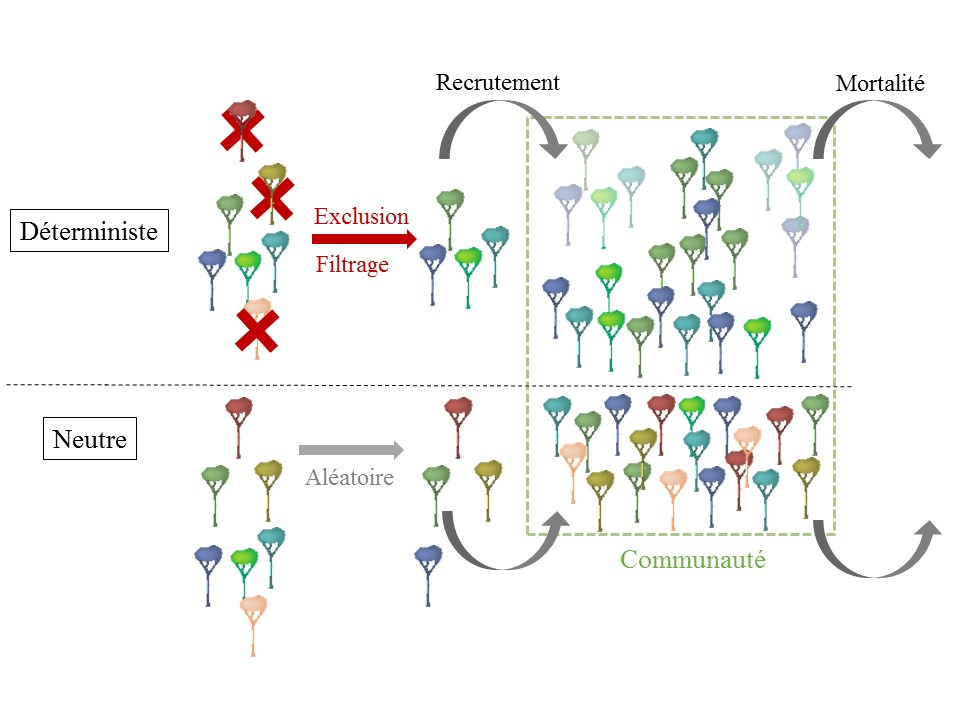
\includegraphics[width=1\linewidth]{ExternalFig/Fig_AssemblyRules} 

}

\caption{Schéma des processus déterminant la réponse des communautés végétales aux perturbations. Les processus déterministes (partie haute) sélectionnent les espèces recrutées dans la communauté selon leurs préférences environnementales e leur compétitivité, tandis que les processus stochastiques (partie basse) reviennent à une sélection aléatoire.}\label{fig:AssemblyRules}
\end{figure*}

\subsection{Les règles d'assemblage des
communautés}\label{les-regles-dassemblage-des-communautes}

Expliciter et comprendre la réponse des forêts aux perturbations
nécessité d'expliciter les processus écologiques sous-jacents. Plusieurs
hypothèses sur les processus d'assemblage des communautés sont débattues
aujourd'hui, notamment quant au rôle des processus stochastiques et
déterministes. Les processus déterministes sélectionnent les espèces de
la communauté selon leur performance dans l'environnement biotique et
abiotique de la communauté , définie par leurs caractéristiques
biologiques \autocite{Molino2001}. Les processus stochastiques, qui
relèvent de la théorie neutre, supposent un assemblage aléatoire
dépendant uniquement de l'histoire de la communauté et des limitations
physique de dispersion ou de croissance (barrière à la dispersion, ordre
d'arrivée des espèces) \ref{fig:AssemblyRules} \autocite{Hubbell2001}.

Le débat quant au rôle respectifs des processus stochastiques et
déterministes est matérialisé dans le cas des forêts tropicales par la
controverse sur la théorie des perturbations intermédiaires
(\emph{Intermediaite Disturbance Hypothesis}, \emph{IDH} en anglais).
Cette théorie suppose la prépondérance de processus déterministes
d'exclusion compétitive et de filtrage des espèces et prédit que, sous
un certain seuil, la diversité est d'autant plus élevée que le milieu
est perturbé \autocite{Molino2001}. Un tel régime de perturbations
intermédaires ferait varier les conditions environnementales sans
engendrer de modification drastique. Cette variabilité permettrait à un
large panel d'espèces de s'installer ou de s'imposer lorsque les
conditions environnementales leur deviennent favorables ou qu'elles
deviennent plus compétitives relativement au reste de la communauté. Au
delà d'un seuil d'intensité de perturbation en revanche les processus de
sélection excluent plus d'espèces qu'ils n'en favorisent et la diversité
des communautés diminue
\autocites{Chesson2000}{Kariuki2006a}{Berry2008a}.

A l'inverse la théorie neutre suppose que les espèces sont équivalentes
et que leur abondance ne dépend pas de leurs caractéritiques
biologiques. L'abondance des espèces dépendrait plutôt de processus
aléatoires de dispersion, de croissance et de survie qui résultent en un
assemblage stochastique des communautés \autocite{Hubbell2001}.

Bien que débattues les hypothèses déterministe et stochastique ne sont
cependant pas incompatibles et ont montré pouvoir prédire la structure
des communautés à différentes échelles et à différents niveaux de
richesse. Il est vraisemblable que les communautés résultent de
combinaisons variables de processus déterministes et stochastiques, et
la question se porte alors sur les facteurs qui influencent l'importance
relative de ces processus \autocite{Chave2004}.

\section{Comment mesurer la diversité biologique
?}\label{comment-mesurer-la-diversite-biologique}

Les processus démographiques et les règles d'assemblage d'espèces
déterminent la structure, la composition et la diversité des
communautés. Prédire et gérer l'avenir des forêts et en particularité de
leur précieuse diversité biologique nécessite de comprendre le rôle des
ces différents processus dans la définission de la diversité biologique
dans tous ses aspects. La biodiversité est définie de l'échelle du gène
à celle de l'écosystème considère la diversité des plantes, animaux,
champignons et microorganismes qui constituent les écosystèmes, de leur
variabilité génétique et phénotypique, et de la variabilité de leurs
assemblages \autocite{Loreau2005}. La biodiversité est souvent réduite à
celle de richesse en espèces, mais tient compte en réalité des multiples
aspects de richesse, d'homogenéité, de disparité et d'interactions entre
les éléments du vivant qui constituent les communautés. Appréhender les
différents aspects de la biodiversité permet d'identifier les mécanismes
écologiques fondamentaux qui régissent les écosystèmes et leurs
dynamiques spatiales et temporelles \autocites{Purvis2000}{Loreau2005}.

\subsection{Composition et dissimilarité entre
communautés}\label{composition-et-dissimilarite-entre-communautes}

De nombreuses mesures permettent d'estimer ce turnover, qui prennent en
compte ou non l'abondance des espèces \autocite{Podani2013}. Nous avons
choisis ici de mesurer le taux de remplacement d'abondance, ou
similarité de Bray-Curtis, qui représente dans quelle mesure une
communauté est le sous-ensemble d'une plus grande. En pratique, si la
communauté recrutée après exploitation répond aux mêmes lois que la
communauté initiale elle sera équivalente à une communauté qui en aurait
été tirée au hasard. La similarité de Bray-Curtis mesure la somme des
abondances d'une commaunté remplacées par une espèce différente,
normalisée par l'abondance totale partagée entre les deux communautés
\eqref{eq:formNestedness}.

\begin{equation}
T_{ab}=\frac{\sum_{i=1}^{n}|x_i^a - x_i^b| - \bigg| \sum_{i=1}^{n}{x_i^a} - \sum_{i=1}^{n}{x_i^b} \bigg|}{\sum_{i=1}^{n}\max{\left( x_i^a;x_i^b \right)}}
\label{eq:formNestedness}
\end{equation}

\subsection{Assemblage et structure des
communautés}\label{AbundanceDistribution}

Une communauté, qu'elle soit végétale, animale ou microbienne, est
constituée d'espèces aux effectifs différents: certaines sont très
abondantes, d'autres moyennement communes et d'autres encore, souvent la
majorité, sont rares. La façon la plus simple et immédiate de décrire
une communauté est de donner la distribution d'abondance de ses espèces,
qui représente les proportions d'espèces abondantes rapport aux espèces
communes ou rares. Cette distribution bien que variable d'une communauté
à l'autre, est régie par des lois écologiques lui donnant invariablement
une courbe en creux \ref{fig:AbdDist} \autocite{McGill2007}.

\begin{figure*}

{\centering 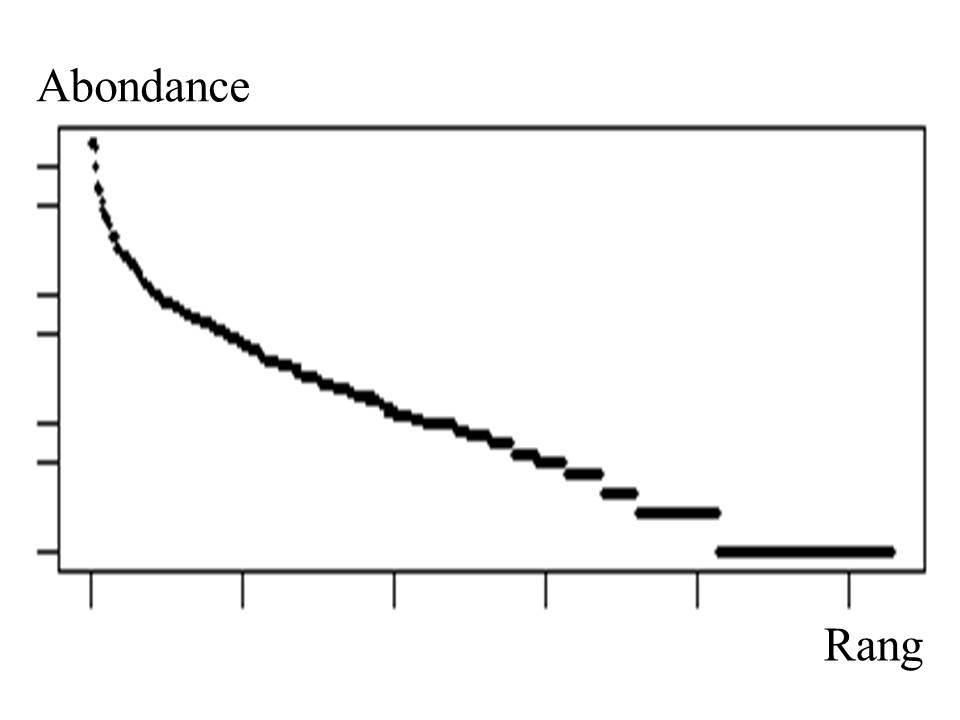
\includegraphics[width=0.6\linewidth]{ExternalFig/SpeciesAbdDist} 

}

\caption{Exemple de distribution d'abondance pour une communauté d'arbres en forêt tropicale humide}\label{fig:AbdDist}
\end{figure*}

Cette uniformité des distributions d'abondance a motivé le développement
de modèles proposant des relations mathématiques entre le nombre
d'espèces et leur abondance. Ces modèles reflètent le lien entre
l'importance d'une espèce dans la communauté et la quantité de
ressources qu'elle mobilise pour son développement: plus une espèce est
compétitive, plus elle sera abondante. Ce lien s'établit vis à vis de la
ressource limitante, qui peut être la lumière, l'eau disponible, les
nutriments du sol, l'espace, etc
\autocites{Silvertown2004}{terSteege2006}. Prédire une distribution
d'abondance revient à prédire la répartition de la ressource limitante
entre les espèces de la communauté. De nombreux modèles prédictifs ont
été proposés, des modèles statistiques divisant aléatoirement la
ressource selon une loi de propabilité donnant les effectifs de chaque
espèce, aux modèles mécanistes divisant la resource selon une formule
prédéterminée, par exemple en la divisant successivement selon une
fraction constante
\autocites{Fisher1943}{Motomura1932}{Tokeshi1993}{Magurran1988}.

Ces modèles testés pour de nombreuses communautés, ont démontré pouvoir
représenter correctement les communautés réelles et révéler les règles
écologiques qui en régissent l'assemblage. Ce sont des outils adéquats
pour comparer les communautés et en interpréter les différences, mais
manipuler une distribution d'abondance reste compliqué car il s'agit
d'une repréentation en 2D et ne permet pas de quantifier les différences
entre communautés. En revanche, les paramètres de ces distributions et
des modèle proposés pour les représenter permettent de quantifier le
nombre d'espèces, la forme des distribution, ou encore l'homogénéité des
abondances. Ces indicateurs sont les indices de diversité, résumant de
façon quantifiable les caractéristiques des distributions d'abondance.

\subsection{Les composantes de la
diversité}\label{les-composantes-de-la-diversite}

Si la biodiversité d'une communauté est souvent assimilée à sa richesse
en espèces, elle englobe en réalité le nombre, l'abondance, la
composition et les interactions entre les espèces. L'abondance en
particulier est essentielle: une espèce dominante n'apportera pas la
même contribution à l'écosystème qu'une espèce rare. Ainsi une
communauté dominée par une ou deux espèces très abondantes sera
intuitivement moins diverse qu'une autre avec autant d'espèces mais aux
abondances équivalentes. L'homogeneité des abondances dans une
population, ou \emph{équitabilité}, peut être bien plus révélatrice du
fonctionnement des écosystèmes que leur richesse ou leur composition.
Cette idée est illustrée par l'hypothèse du ratio de biomasse selon
laquelle les espèces dominantes sont bien plus déterminantes du
fonctionnement des écosystèmes que les espèces rares. Les espèces peu
communes n'ont une influence qu'à long terme, en tant que potentielles
futures espèces dominantes si l'environnement change, ou pas d'influence
si elles sont transitoires et ne persistent pas dans l'écosystème
\autocite{Grime1998}.

La richesse, simplement le nombre d'espèces recensées, et
l'équitabilité, la régularité de distribution d'abondance des espèces,
sont donc les deux composantes de la diversité taxonomique d'une
communauté \ref{fig:RichEqu} \autocites{Whittaker1965}{Magurran2004}.

\begin{figure*}

{\centering 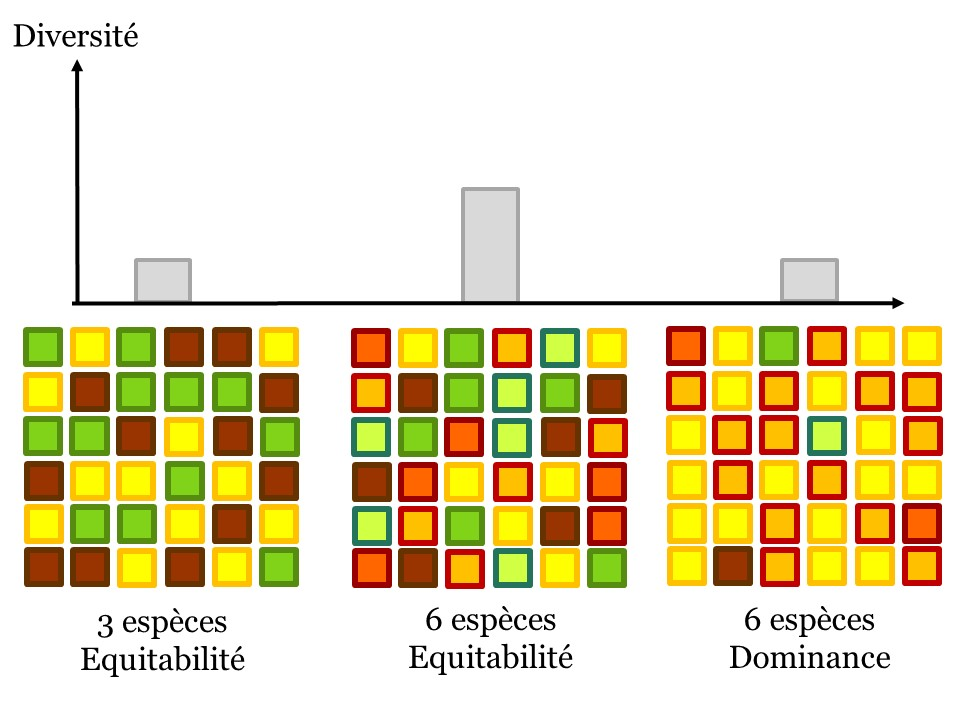
\includegraphics[width=0.6\linewidth]{ExternalFig/Fig_RichnessEquitability} 

}

\caption{Les deux composantes de la diversité taxonomique: richesse (nombre d'espèces) et équitabilité (homogeneité de répartition)}\label{fig:RichEqu}
\end{figure*}

Mesurer la diversité ne revient donc pas à une mesure unique mais
plusieurs indices de diversité qui combinent différemment les
composantes de la diversité. Plusieurs familles d'indices de diversité
ont été développées et regroupent les indices mesurés selon une même
formule dont les déclinaisons accordent un poids variables aux
composantes de la diversité. La famille des indices de diversité de
Réyni par exemple, judicieuse pour l'étude des communautés végétales,
rassemble les indices mesurés selon l'équation \eqref{eq:formHCDT} modulée
par un paramètre \emph{q} appelé ``ordre de diversité'' qui correspond
au poids des espèces rares par rapport aux espèces abondantes
\autocite{Mendes2008}. Plus l'ordre de diversité est élevé, plus les
espèces rares sont négligées par rapport aux espèces abondantes.

\begin{equation}
{^{q}H=\frac{1}{q-1}\Bigg(1-\displaystyle\sum_{s=1}^{S}p^q_s\Bigg) }
\label{eq:formHCDT}
\end{equation}

Dans cette famille d'indices de diversité se retrouvent les indices les
plus utilisés dans la littérature: l'ordre 0 où chaque espèce contribue
de la même façon correspond à la richesse spécifique, l'ordre 1 où
richesse et équitabilité sont également prises en compte correspond à
l'indice de Shannon, et l'ordre 2 pour lequel les espèces rares sont
presque négligées correspond à l'indice de Simpson (parfois appelé
``diversité en espèces abondantes'')
\autocites{Shannon1948}{Simpson1949}{Patil1982}{Tothmeresz1995}.

Ces indices, mathématiquement corrects et représentatifs des différentes
composantes de la diversité, ne donnent cependant pas un nombre
intelligible qui permettent de comparer facilement différentes
communautés. Les indices de diversité doivent être traduits en
\emph{nombre équivalent d'espèces} qui correspond au nombre d'espèces
qu'aurait la communauté étudiée si toutes les espèces avaient la même
abondance. Ce nombre équivalent d'espèces, ou \emph{nombre de Hill}, est
obtenu par transformation des valeurs obtenues par une exponentielle à
base q \autocite{Hill1973}.

Les mesures de diversité choisies sont donc la traduction intelligible
en nombre équivalent d'espèces d'une déclinaison d'indices combinant
richesse et équitabilité de différentes façons pour capter toute
structure de diversité.

\subsection{Résolution du biais
d'échantillonnage}\label{resolution-du-biais-dechantillonnage}

En pratique aucun inventaire n'est exhaustif et l'étude de la diversité
se heurte aux biais d'échantillonnage qui sous-estiment la richesse et
faussent l'abondance des espèces. Corriger ce biais nécessite d'estimer
les abondances réelles à partir des observations et des relations
mathématiques reliant les abondances des différentes espèces. La
première méthode développée correspond à la formule des fréquences de
Turing \autocite{Good1953} où l'abondance réelle *\alpha\_v* d'une
espèce observée \emph{v} fois dans un échantillonnage de \emph{n}
individus dépend du nombre d'espèces observées également \emph{v} fois
et d'e celles'espèces observées \emph{v+1} fois
@ref\{eq=formGoodTuring\}:

\begin{equation}
\alpha_v=\frac{\big(v+1\big)}{n}\frac{s^n_{v+1}}{s^n_v}
\label{eq:formGoodTuring}
\end{equation}

Les singletons (espèces observées une seule fois) et les doubletons
(espèces observées deux fois) sont alors particulièrement intéressants
car il permettent d'estimer le nombre \emph{s\^{}n\_0} d'espèces
observées zéro fois (\(s^n_0=\frac{s^n_1}{n}\)) qui ont été manquées
dans l'inventaire et peuvent être ajoutées aux observation pour corriger
le biais d'échantillonnage de la richesse.

De nombreuses méthodes ont repris cette relation en y intégrant
notamment la notion de \emph{taux de couverture} qui quantifie l'effort
d'échantillonnage d'un inventaire réel et permet de savoir quelle
proportion de la communauté est échantillonnée \autocite{Dauby2012}. La
correction la plus adéquate a pu être déterminée selon le taux de
couverture de l'inventaire et les estimateurs de la diversité sont
aujourd'hui très fiables \autocites{Chao2015}{Marcon2015b}.

\subsection{Diversité fonctionnelle}\label{diversite-fonctionnelle}

Les mesures de diversité décrites précédemment, appelées diversité
neutre, considèrent toutes les espèces de la même façon que celles-ci
aient ou non des caractéristiques biologiques ou phylogénétiques
proches. Ces diversités peuvent cependant facilement intégrer les
caractéristiques des espèces en mesurant leur similarité et une
communauté sera d'autant plus diverse que les espèces qui la constituent
sont différentes. Pour des communautés végétales la diversité
phylogénétique considère les distances entre espèces dans un arbre
phylogénétique et la diversité fonctionnelle considère leurs différences
morphologiques ou physiologiques \ref{fig:RichEquSim}.

\begin{figure*}

{\centering 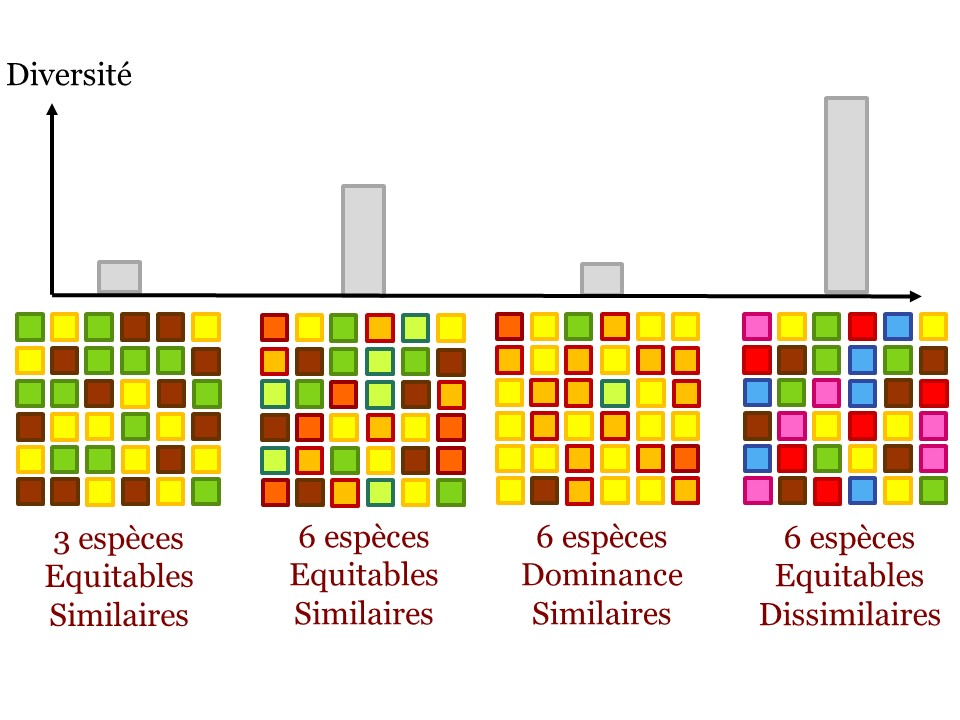
\includegraphics[width=0.6\linewidth]{ExternalFig/Fig_RichnessEquitabilitySimilarity} 

}

\caption{Troisième composante de la diversité: la similarité entre espèces basée sur des distances phylogénétiques ou taxonomiques}\label{fig:RichEquSim}
\end{figure*}

Ces similarités sont ensuite intégrées aux indices de diversité, au même
titre que la richesse et l'équitabilité, sous la forme d'une matrice de
distances entre espèces calculée sur la base de leur phylogénie ou de
leurs traits fonctionnels.

Les traits fonctionnels sont les caractéristiques morphologiques,
physiologiques et phénologiques des espèces, ils déterminent le
fonctionnement des individus, leur performance de croissance et de
survie, et leurs interaction avec l'environnement
\autocite{Violle2007b}. L'approche fonctionnelle décrivant les espèces
et les individus selon leurs caractéristiques biologiques a été
largement adoptée en écologie. D'une part, cette approche réduit la
dimensionnalité des communautés, indispensable pour l'étude
d'écosystèmes aussi riches que les forêts tropicales et permet de
comparer les communautés quelle que soit leur composition en espèces
\autocites{Begon2006}{Scheiter2013}{Mouillot2013a}{Sakschewski2016}.
D'autre part, composition et diversité fonctionnelle sont interprétables
en termes d'utilisation des ressources et de flux de matière et
d'énergie, et relient directement la diversité des communautés à leur
fonctionnement. Enfin, cette approche appréhende la signature
fonctionnelle des perturbations et permet d'identifier et de quantifier
les processus déterminant la dynamique des communautés
\autocite{Funk2017}. La définition des processus déterministes est
qu'ils n'impliquent pas les espèces de la même façon selon leurs
caractéristiques biologiques: l'exclusion abiotique d'espèces non
adaptées à l'environnement se traduiront par une aggrégation de la
communauté dans l'espace des traits fonctionnels et une diminution de sa
diversité fonctionnelle, tandis que l'exclusion compétitive limitant les
similarité entre espèces se traduira par une dispersion des traits
fonctionnels de la communauté et une diversité fonctionnelle élevée
\autocites{McGill2006}{Kunstler2012}.

L'approche fonctionnelle nécessite de choisir judicieusement les traits
intégrés aux indices de diversité. Une vaste littérature a permis
d'identifier les traits clés représentatifs de l'écologie et de la
croissance des espèces et de leur influence sur le fonctionnement de
l'écosystème \autocite{Reich2014}. Les traits foliaires tout d'abord,
qui déterminent la stratégie d'acquisition et d'allocation des resources
lumineuses, définissent un ``spectre économique foliaire'' qui oppose
les espèces à larges feuilles fines ayant une forte capacité
photosynthétique permettant une acquisition rapide des resources, aux
espèces à petites feuilles coriaces et résistantes. Un gradient
similaire s'applique aux traits racinaires et aux propriétés du bois,
opposant les espèces aux tissus légers à courte durée de vie permettant
une croissance rapide à celles aux tissus denses plus résistants et
mobilisant plus de ressources
\autocites{Chave2009}{Valverde-Barrantes2017}. Les stratégies
d'acquisition des resources déterminent la stratégie de croissance des
espèces: les espèces ``acquisitives'' auront une croissance rapide et
une courte durée de vie tandis que les espèces ``conservatives'' auront
une croissance plus lente mais une meilleure résistance aux conditions
environnementales éprouvantes \autocites{Reich1997}{Wright2004}. A ces
traits fonctionnels mesurables à l'échelle de l'individus s'ajoutent des
\emph{traits d'histoire de vie} mesurables à l'échelle de l'espèce.
Parmi ces traits la masse des graines et la hauteur moyenne maximale des
arbres à l'âge adulte ont montré être particulièrement représentatifs
des stratégies de croissance, de survie et de reproduction
\autocites{Westoby1998}{Herault2011}. La combinaison de l'ensemble de
ces traits spécifique, foliaires, racinaires et du bois appréhende la
stratégie fonctionnelle des espèces, leurs préférences écologiques et
leur performance de croissance et de survie. L'engouement récent de
l'écologie pour l'approche fonctionnelle a de plus permis la création de
bases de données fonctionnelles conséquentes et standardisées qui
rendent possibles l'approche fonctionnelle à l'échelle des communautés
{[}\textcite{Kattge2011}; \textcite{Perez-Harguindeguy2013}; \footnote{\url{http://www.ecofog.gf/Bridge/}}{]}

L'approche fonctionnelle considère la diversité des communautés mais
également leur composition fonctionnelle mesurable par les valeurs
moyennes de traits pondérées par l'abondance des espèces
(\emph{Community Weighted Means, CWM} en anglais). L'abondance des
caractéristiques fonctionnelles détermine à la fois le fonctionnement
des communautés et leur résilience. D'après la théorie du ``ratio de
biomasse'' \autocite{Grime1998}, le rôle d'un individu dans l'écosystème
dépend de la fraction de biomasse qu'il représente et le fonctionnement
des communautés repose sur les espèces dominantes tandis que les espèces
rares ont peu d'influence.

Par ailleurs la répartition d'abondance des traits fonctionnels amène à
la notion de redondance fonctionnelle qui quantifie le nombre d'espèces
partageant les mêmes valeurs de traits. La redondance fonctionnelle,
souvent élevée en forêt tropicale, permet aux communautés de perdre des
espèces sans nécessairement voir disparaître leur rôle dans
l'écosystème: la redondance détermine en partie la résilience des
communautés et atténue l'impact des perturbations. L'organisation de la
redondance dans l'espace des traits d'une communauté renseigne sur les
assemblages les plus stables qui se dégageraient le plus probablement
après de nouvelles perturbations. La redondance fonctionnelle d'une
communauté peut se mesurer dans l'espace fonctionnel à partir de la
densité de probabilité de traits (\emph{Traits Density Probability, TDP}
en anglais) de chaque espèce \autocite{Carmona2016}. Les densités des
espèces d'une communauté pondérées par leur abondance sont additionnées
pour donner la redondance fonctionnelle sur l'ensemble de l'espace
fonctionnel ou sur un espace restreint, comme nous le ferons par la
suite quand on s'intéressera à la redondance fonctionnelle dans l'espace
de la communauté de départ \ref{fig:RedundancyMethod}.

\begin{figure*}

{\centering 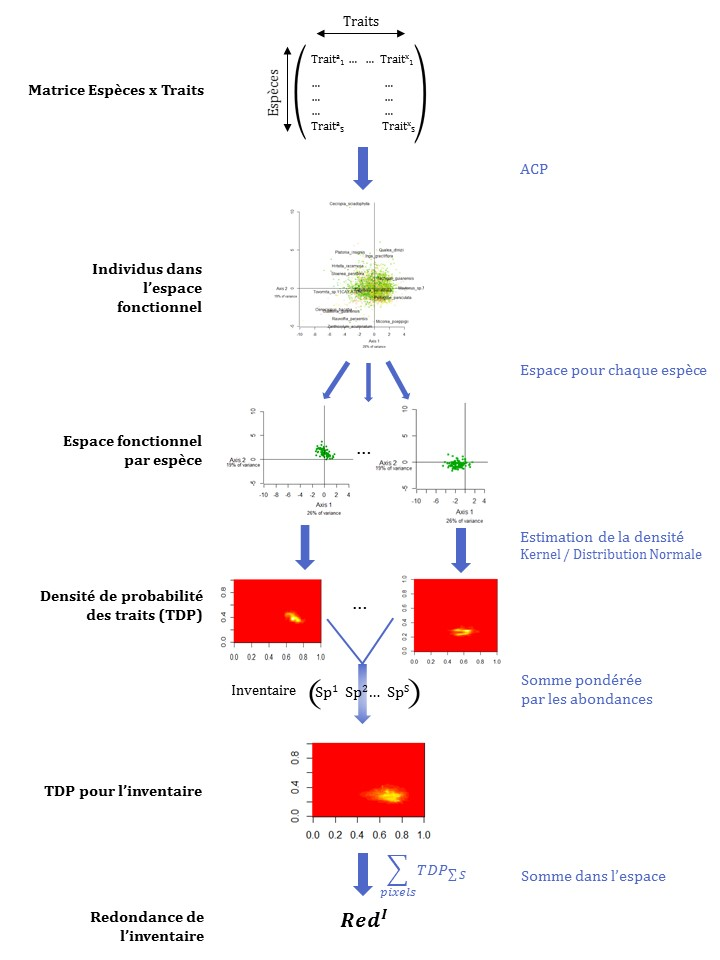
\includegraphics[width=1\linewidth]{ExternalFig/Fig_MesureRedondance} 

}

\caption{La redondance fonctionnelle est la somme des chevauchement entre espèces dans l'espace fonctionnel. Les individus de la base de données fonctionnelle sont représentés dans un espace à 2 dimensions grâce à une analyse en composantes principales (ACP). Une estimation par noyau estime ensuite la densité de probabilité des traits (TDP) de chaque espèce. La somme de ces densités pondérées par l'abondance des espèces donne enfin la redondance fonctionnelle de la communauté, interprétable comme le nombre d'espèces qui peuvent disparaître sans diminuer l'espace fonctionnel de la communauté.}\label{fig:RedundancyMethod}
\end{figure*}

\section{La Guyane Française et l'exemple de la station de
Paracou}\label{la-guyane-francaise-et-lexemple-de-la-station-de-paracou}

Le bassin Amazonien est la plus riche des trois principales régions de
forêt tropicale humide \autocite{Gentry1988} et la Guyane française en
est une région de 83 846 km\textsuperscript{2} recouverte à 95\%
forestière au Nord-Est du continent sud-américain entre le Surinam et le
Brésil.

\subsection{Le contexte Guyanais}\label{le-contexte-guyanais}

La région appartient au bouclier des Guyanes qui s'étend de l'Amapa au
Brésil jusqu'au delta de l'Orénoque au Venezuela. Formé il y a plus de 2
milliards d'années, le bouclier des Guyanes est un assemblage d'unités
géomorphologiques façonnées par une succession d'épisodes géologiques,
climatiques et marins. Ces unités correspondent à des conditions
pédologiques, climatiques et topographiques déterminant la composition
et la diversité du couvert végétal et les processus écologiques qui les
régissent, tels que les migrations et le filtrage environnemental
\autocite{Guitet2015}.

Le relief Guyanais est une grande diversité topographique qui alterne
entre des collines allant jusqu'à 50m d'altitude, et des bas-fonds
humides. Les sols sont des Acrisols recouvrant une couche de saprolite
transformée peu perméable qui entraîne un drainage latéral des
précipitations. La profondeur des sols, leur composition et leur
capacité de rétention et de drainage de l'eau sont très hétérogènes
\autocites{Ferry2010}{Robert2003}.

Le climat est un climat tropical humide, davantage marqué par le régime
des précipitations que par celui des températures. La température
moyenne est 26°C et reste constante au cours de l'année tandis les
précipitations moyennes annuelles varient de 2 000 à 4 000
mm.an\textsuperscript{-1} et montrent une grande variabilité spatiale et
temporelle. Les précitations suivent un gradient décroissant marqué
d'est en ouest et une forte variabilité au cours de l'année, avec une
saison humide entre novembre et avril et une saison sèche d'avril à
mi-juillet durant laquelle les précipitations sont inférieures à 50 mm
\autocite{Wagner2011}.

La forêt Guyanaise est une forêt équatoriale sempervirente ombrophile de
plaine. D'une richesse incroyable, elle accueille plus de 7 000 espèces
végétales (hors champignons) dont 1 500 espèces d'arbres et une richesse
faunistique toute aussi incroyable \autocite{DeNoter2008}. La
composition taxonomique des arbres est très variable sur le territoire.
Plusieurs patrons de composition on été mis en évidence selon un
gradient du nord-ouest où dominent les familles botaniques des
\emph{Lecythidaceae} et \emph{Cesalpinaceae}, au sud-est où dominent
\emph{Burseraceae} et \emph{Mimosaceae}. Ces patrons suivent en
particulier par une combinaison de gradients topographique et
pédologique \autocites{Sabatier1989}[ cf
Toto]{Sabatier1997}{Guitet2015}.

\subsection{Paracou, plus de 30 de suivi de la forêt
Amazonienne}\label{paracou-plus-de-30-de-suivi-de-la-foret-amazonienne}

Le dispositif de Paracou, installé entre les communes de Kourou et
Sinnamary (5°18'N and 52°53'W), a été mis en place en 1984 pour étudier
l'impact de l'exploitation forestière sélective sur les peuplements
forestiers. Le dispositif correspond à l'origine à 12 parcelles de 6.25
ha ayant subi en 1984 un gradient de trois intensités d'abattage,
d'éclairices et de coupe de bois de chauffage. Le traitement de
perturbation a été attribué selon un dispositif aléatoire de trois
réplications de 4 traitements: parcelles témoins sans intervention
(\emph{T0}), traitement 1 avec coupes d'abattage (\emph{T1}), traitement
2 avec abattage et éclaircies par annélation (\emph{T2}), traitement 3
avec abattage, éclaircies et coupe de bois de chauffage (\emph{T3})
\ref{tab:InterventionTable}.

En 1990, trois parcelles de 6.25ha et une parcelle de 25ha (parcelles
13, 14, 15 et 16) ont été ajoutées au dispositif pour l'étude et le
suivi de la diversité en forêt non perturbée \ref{fig:ParacouDesign}.

\begin{figure*}

{\centering \includegraphics[width=0.6\linewidth]{ExternalFig/Paracou} 

}

\caption{Dispositif expérimental de Paracou, schéma des 16 parcelles de suivi des dynamiques forestières. La couleur des parcelles indique l'intensité de perturbation appliquée à 9 des parcelles en 1984 (voir le tableau 1.}\label{fig:ParacouDesign}
\end{figure*}

Sur l'ensemble du dispositif sont recensées 591 espèces d'arbres
appartenant à 223 genre et 64 familles botaniques, principalement les
\emph{Fabaceae}, les \emph{Chrisobalanaceae}, les \emph{Lecythidaceae}
et les \emph{Sapotaceae}. Les températures annuelles atteignent 26°C et
les précipitations 2 980 mm.an\textsuperscript{-1} de mi-août à
mi-novembre, avec une saison sèche d'un mois en mars
\autocite{Wagner2011}.

\subsection{Méthodes d'inventaires}\label{methodes-dinventaires}

Depuis la mise en place du dispositif en 1984 toutes les parcelles sont
inventoriées chaque année à la saison sèche à partir de mi-juillet. Tous
les arbres de plus de 10 cm de diamètre à 1.30 m (diamètre à hauteur de
poitrine, \emph{DBH} en anglais) sont identifiés, numérotés et
cartographiés. Les arbres morts sont relevés chaque année et notés en
précisant le type mort (mort sur pied, chablis primaire ou chablis
secondaire).

Lorsqu'un arbre atteint 10 cm il est \emph{recruté} et sera mesuré
chaque année. Il est identifié dans un premier temps par un nom
\emph{vernaculaire}, ou nom commun, attribué par l'équipe de terrain. En
1984, 62 espèces commerciales étaient identifiées par un nom commun
propre tandis que toutes les autres espèces étaient regroupées sous deux
noms vernaculaires distinguant les palmiers des espèces arborées. Cette
identification en nom vernaculaire s'est précisée par la suite et
aujourd'hui 235 noms vernaculaires différents sont recensés pour
l'ensemble du dispositif sur les 30 ans de suivi. Des campagnes
d'identification botanique au cours desquelles les arbres sont
identifiés au niveau espèce botanique ont été mises en place à partir de
2003 et se poursuivent depuis tous les 5 à 6 ans.

L'histoire des inventaires botaniques s'étant construite petit à petit
au gré des nouveaux projets et des forces en présence, la précision et
le taux d'identification botaniques sont variables au cours du temps et
entre les parcelles. Ceci génère des incertitudes taxonomiques
importantes, les noms vernaculaires correspondant souvent à plusieurs
noms botaniques et inversement \autocite{Oldeman1968}. Le soucis vient
alors des arbres n'ayant qu'un identification en nom vernaculair,
lorsque l'individu est mort avant d'avoir pu être identifié au cours
d'une campagne botanique par exemple.

\section{Problématique et plan de la
thèse}\label{problematique-et-plan-de-la-these}

La thèse présentée ici cherche à déterminer les processus écologiques et
la réponse taxonomique et fonctionnelle après perturbation d'une forêt
tropicale naturelle et à expliciter sa résilience, en vue de discuter de
son maintien dans le contexte actuel des changements globaux et de la
possibilité d'une sylviculture durable. Le document s'organise en trois
chapitres correspondant à trois articles scientifiques en cours de
soumisson.

\begin{itemize}
\item
  Le premier chapitre présente un estimateur de la diversité taxonomique
  et fonctionnelle des communautés tenant compte des incertitudes
  taxonomiques inhérentes aux inventaires forestiers. La méthode utilise
  l'association entre noms vernaculaires et noms botaniques pour
  reconstituer itérativement des inventaires complets théoriques à
  partir desquels sont estimés moyenne et l'intervalle de sûreté de la
  diversité. Dans un premier temps nous calibrons la méthode pour avoir
  l'estimation la plus précise possible en fonctoin des données
  disponibles. Dans un deuxième temps nous appliquons la méthode de
  propagation au cas des inventaires forestiers, qui couvrent de larges
  surfaces de temps et d'espace, pour les valoriser dans l'étude et la
  préservation des forêts tropicales. Enfin nous appliquons cette
  méthode aux dispositifs expérimentaux, dont les contraintes
  d'incertitude sont différentes, et qui sera utilisée dans la suite de
  ce travail.
\item
  Dans le deuxième chapitre nous avons étudié les trajectoires de
  composition et de diversité taxonomique et fonctionnelle des 75ha de
  Paracou suivis sur 30 ans. Ces trajectoires permettent de clarifier la
  réponse aux perturbations de la composition et la diversité des
  communautés en forêts Néotropicale, d'identifier les processus
  écologiques sous-jacents, et de discuter de leur résilience.\\
  Nous examinons en particulier (i) la convergence des trajectoires
  taxonomiques et fonctionnelles et leur implication quant au maintien
  des différences entre communautés après perturbation, (ii) la validité
  théorie des perturbations intermédiaires, débattue en forêt tropicale
  et rarement testée sur le long terme, et (iii) la durée et aspects de
  la résilience des communautés.
\item
  Dans le troisième chapitre nous étudions spécifiquement les
  trajectoies de recrutement. Nous testons en particulier (i) la
  déclinaison des modèles classique de succession forestière pour forêts
  tropicales, dont la validité est questionnée par l'immense diversité
  des communautés, et après une perturbation modérée, qui implique la
  maintient d'une communauté pre-perturbation significative, et (ii)
  questionnons la durée de restauration du fonctionnement de
  l'écosystème et les implications pour la gestion forestière.
\end{itemize}

\chapter{Article 1 : Des inventaires forestiers aux trajectoires de
diversité: le problème universel de
l'incertitude}\label{article-1-des-inventaires-forestiers-aux-trajectoires-de-diversite-le-probleme-universel-de-lincertitude}

Malgré les enjeux liés aux forêts tropicales et l'urgence d'en préserver
l'intégrité et le fonctionnement, seule une petite fraction de leur
diversité est connue. Le nombre d'espèces inventoriées sous les
tropiques ne correspondant qu'à une observation unique
\autocite{Feeley2011} présume de l'ampleur de notre méconnaissance et
rend impossible toute supposition sur la distribution des espèces et
leurs dynamiques. Il est essentiel d'améliorer notre connaissance du
vivant, en fournissant un plus grand effort d'échantillonnage et en
valorisant toute connaissance déjà disponible.

Le coût des inventaires en temps, en main d'oeuvre et en moyens,
d'autant plus important que le niveau de l'inventaire est précis,
implique de travailler également à des méthodes pour valoriser tout type
d'inventaires \autocite{Baraloto2012}. Dans le cas de l'étude des
peuplements forestiers, les inventaires d'exploitation peu coûteux et
couvrant des surfaces larges sont une source d'information
incontournable \autocites{terSteege2000}{Guitet2014}.

\section{Noms vernaculaires et propagation des incertitudes
taxonomiques}\label{noms-vernaculaires-et-propagation-des-incertitudes-taxonomiques}

Ces inventaires ne sont cependant généralement pas réalisés en noms
scientifiques mais noms vernaculaires, qui sont mieux connus, plus
faciles à attribuer car basés sur des critères morphologiques, culturels
ou d'usage et qui ne nécessitent pas de vérification botanique
ultérieure à partir d'herbiers. Cette simplicité se fait cependant au
détriment de la fiabilité des noms vernaculaires, qui correspondent à
plusieurs espèces botaniques et varient avec le temps et les équipes de
terrain \autocite{Oldeman1968}. Nous proposons ici une méthode de
propagation des incertitudes taxonomiques permettant d'estimer la
diversité des communautés en palliant les indéterminations botaniques.
La méthode se base sur la reconstitution d'inventaires complets
théoriques à partir des associations entre noms vernaculaires et
botaniques.

Dans un premier temps nous avons déterminé la source la plus fiable pour
calculer les associations entre noms vernaculaires et botaniques. Ces
associations peuvent effectivement être estimées à partir d'inventaires
réels ou à partir de dires d'experts, les ouvriers forestiers qui
réalisent les inventaires et fournissent une liste des associations
connues.

Dans un deuxième temps nous appliquons la méthode de propagation au cas
des inventaires forestiers réels qui, réalisés à large échelle dans le
cadre de l'exploitation, permettraient d'élargir l'étude de la
biodiversité forestière dans le temps et l'espace s'ils étaient plus
précis. La précision des inventaires peut être améliorée par la méthode
de propagation des incertitudes et nous en proposons une application
optimisée. Nous avons testé la précision de l'estimateur de diversité en
fonction de l'effort d'identification botanique (pourcentage d'espèces
identifiées) et de l'effort d'échantillonnage (pourcentage de la surface
couverte), et avons déterminé une méthode d'inventaire optimale.

Enfin, nous adaptons la méthode au contexte des dispositifs
expérimentaux pour pallier la variabilité des pratiques d'inventaires.
Dans le cas des inventaires forestiers pour lesquels l'ensemble des
individus d'une espèce sont indéterminés. Dans le cas des dispotifs
expérimentaux en revanche les indéterminations sont des individus
n'ayant pas été identifié en nom botanique, que l'identification soit
impossible ou qu'ils soient mort avant le passage du taxonomiste. Le
degré d'indétermination correspond alors au nombre d'arbres sans
identification botanique et concerne potentiellement toutes les espèces
de la communauté.

\section{Article 1 \_ Inescapable Taxonomists: Workable Biodiversity
Management Must Base on a Minimum Field
Work}\label{article-1-_-inescapable-taxonomists-workable-biodiversity-management-must-base-on-a-minimum-field-work}

\section{La recherche et les suivis à long terme: application de la
méthode de propagation aux inventaires de
Paracou}\label{la-recherche-et-les-suivis-a-long-terme-application-de-la-methode-de-propagation-aux-inventaires-de-paracou}

\subsection{Profils d'incertitude
taxonomique}\label{profils-dincertitude-taxonomique}

A la différence des inventaires d'exploitation, dans le cas des
dispositifs expérimentaux le degré d'indétermination taxonomique
correspond à un pourcentage d'arbres, toutes espèces confondues, n'ayant
pas été identifiés au niveau spécifique. Sur le même principe que pour
les inventaires d'exploitation, nous avons simulé un gradient
d'indétermination taxonomique à partir d'inventaires complets en nom
botanique complets évaluer l'impact de l'incertitude taxonomique pour
les mesures de diversité \ref{fig:FigTreesSp}.

\begin{figure*}

{\centering 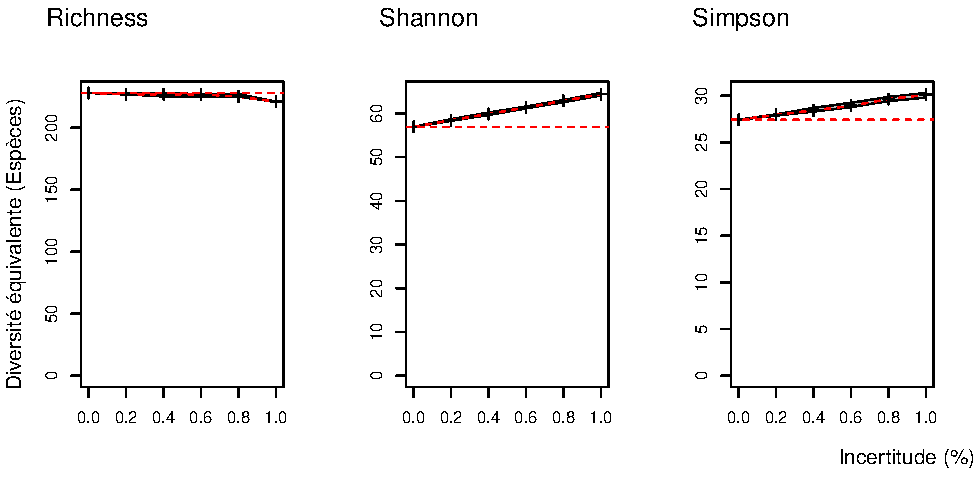
\includegraphics[width=1\linewidth]{MyBook_files/figure-latex/FigTreesSp-1} 

}

\caption{Profil de biais pour les diversité de Richesse, Shannon et Simpson au niveau spécifique le long d'un gradient d'indétermination correspondant au pourcentage d'individus identifiés uniquement par leur nom vernaculaire. Les profils de biais représentent la moyenne et les quantiles 0.025 et 0.975 de la distribution des diversités obtenues pour 100 simulations de tirage aléatoire et de propagation des incertitudes.}\label{fig:FigTreesSp}
\end{figure*}

Le profil de biais obtenu montre un effet non négligeable du degré
d'indétermination sur la mesure de la diversité. L'estimateur de la
richesse reste peu biaisé tant que le degré d'indétermination ne dépasse
pas 80\%, ce qui signifique que toutes les espèces sont représentées par
au moins un individu identifié au niveau botanique. En revanche les
diversités de Shannon et Simpson, et donc l'équitabilité des
communautés, sont significativement surestimées et ceci
proportionellement au degré d'indétermination.

La propagation des incertitudes tend donc à homogénéiser les abondances
de la communauté: les individus indéterminés tirés aléatoirement ont
plus de chances de orrespondre à une espèce abondante (par définition
plus fréquente) et d'être réattribuée par la méthode de propagation à
une espèce plus commune. Le biais semble donc difficile à formaliser car
il dépend de la relation entre rareté et probabilité d'indétermination
des espèces, qui est déterminée par la connaissances botaniques de
l'équipe d'identification.

Pour pallier ce biais nous avons choisis de nous rapporter au niveau
taxonomique supérieur et d'étudier la diversité des communautés en genre
botanique. Le biais de l'estimateur de diversité au niveau espèce est
bien moins important, ne dépassant pas 10\% de la diversité observée
\ref{fig:FigTreesGenus}. Par ailleurs, les estimateurs sont peu
variables et permettent de comparer correctement les communautés
communautés, pourvu que leurs degrés d'indétermination soient
similaires.

\begin{figure*}

{\centering 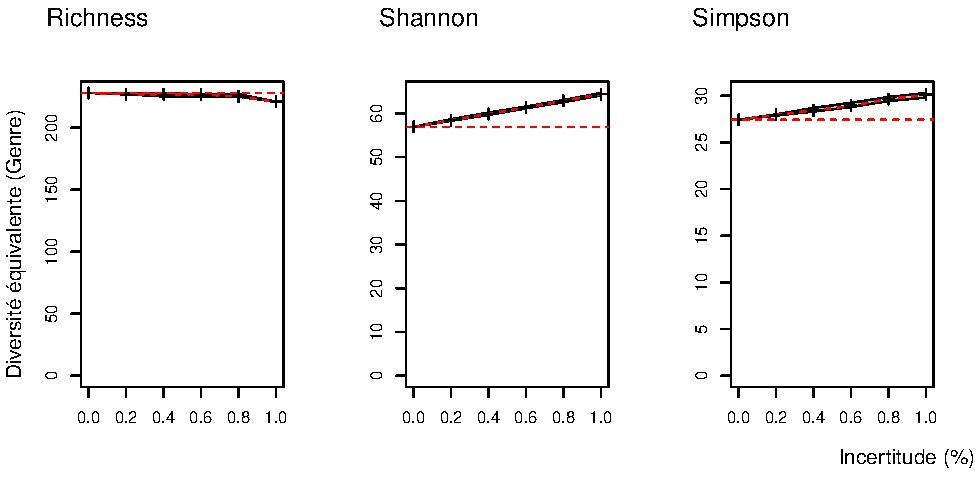
\includegraphics[width=0.6\linewidth]{MyBook_files/figure-latex/FigTreesGenus-1} 

}

\caption{Profil de biais pour les diversité de Richesse, Shannon et Simpson au niveau genre le long d'un gradient d'indétermination correspondant au pourcentage d'individus identifiés uniquement par leur nom vernaculaire. Les profils de biais représentent la moyenne et les quantiles 0.025 et 0.975 de la distribution des diversités obtenues pour 100 simulations de tirage aléatoire et de propagation des incertitudes.}\label{fig:FigTreesGenus}
\end{figure*}

\subsection{Cas particulier de
Paracou}\label{cas-particulier-de-paracou}

L'histoire de détermination botanique des parcelles de Paracou implique
une grande variabilité du degré d'indétermination au cours du temps et
des différences significatives entres les parcelles. Aujourd'hui tandis
que les parcelles contrôle et du traitement 3 sont bien déterminées,
moins de 5\% des arbres 'ne sont identifiés que par un nom
vernaculaire'ont pas d'identification botanique, d'autres parcelles du
traitement 1 ou 2 sont encore mal déterminées et pour certaines plus de
30\% des arbres n'ont pas d'identification botanique.

Jusqu'à présent le biais des estimateurs de diversité reste à resoudre,
en revanche il est possible de pallier ces différences de détermination
en considérant la compositon et la diversité des parcelles au niveau du
genre plutôt qu'au niveau de l'espèce.

\chapter{Article 2: trajectoires de diversité des
parcelles}\label{article-2-trajectoires-de-diversite-des-parcelles}

L'immense biodiversité des forêts tropicales est supposée déterminée et
maintenue par un régime de perturbations régulier, comme l'illustre la
théoriqe des perturbations intermédiaires. Cette théorie suppose une
diversité maximale des communautés pour un régime de perturbation moyen,
mais elle reste débattue dans le cas des forêts tropicales, et cette
controverse conduit à questionner la résilience des communautés après
perturbation.

Nous étudions dans ce chapitre les trajectoires de diversité et de
composition des communautés au cours des 30 années suivant un gradient
de perturbation (10 à 60\% de biomasse prélevée). Nous avons analysé les
trajectoires de composition, de richesse et de redondance taxonomique et
fonctionnelle, en considérant 7 traits fonctionnels des feuilles, du
bois et d'histoire de vie.

Les trajectoires de diversité ont mis en évidence une réponse
taxonomique et fonctionnelle cyclique après perturbation, conduisant à
la restauration des charactéristiques d'avant perturbation. Les
différentes trajectoires ont montré d'une part la divergence taxonomique
des communautés, maintenant leurs différences de composition après
exploitation du fait des limites de dispersion des espèces, et d'autre
part leur convergence fonctionnelle,révélant une réponse commune régie
par des processu de sélection fonctionnels. La théorie des perturbations
intermédiaires a pu représenter correctement l'impact des perturbations
sur la diversité taxonomique, dont l'augmentation est positivement
corrélé à l'intensité de la perturbation jusqu'à un ertain seuil. En
revanche la sélection d'espèces fonctionnellement différentes augmentait
la diversité fonctionnelle après perturbation quelle qu'en soit
l'intensité, l'impact négatif de la perturbation étant atténué par
l'importante redondance fonctionnelle des communautés. Bien
qu'effective, la restauration des charactéristiques taxonomiques et
fonctionnelles des communautés restait inachevée après 30 ans, suggérant
un temps de restauration long de plusieurs décenies d'autant plus
difficile à estimer que la restauration de la redondance fonctionnelle,
déterminante de la résilience des communautés, s'est montrée ralentir au
cours du temps.

\chapter{Article 3: Analyse du recrutement, support de la trajectoire
des
communautés}\label{article-3-analyse-du-recrutement-support-de-la-trajectoire-des-communautes}

La réponse des communautés aux perturbations est déterminée par les
trajetoires du recrutment, reconnu pour suivre une succession
déterministe régie après perturbation. Ceci reste cependant à tester
dans le cas des forêts tropicales, dont l'immense biodiversité pourrait
atténuer les processus déterministes, et dans le cas particulier de
perturbations relativement peu intenses en comparaison des coupes rases
ou de la secondarisation pour lesquels ont été observés les modèles de
succession classique.\\
Nous étudions dans ce chapitre les trajectoires de diversité taxonomique
et fonctionnelle du recrutement après exploitation pour (i) clarifier
l'importance respective des processus stochastiques et déterministes au
cours de la succession des processus écologiques et (ii) déterminer la
résilience et la durée de restauration des processus démographiques
après exploitation.

Nous avons tracé et comparé à des odèles nuls stochastiques les
trajectoires de diversité et d'équitabilité taxonomique, de
renouvellement des espèces par rapport à la communauté avant
perturbation, et de diversité fonctionnelle.

Nous avons identifié trois phases de recrutement après perturbation,
définies par l'équilibre entre les processus déterministes et
stochastiques impliqués. Dans un premier temps les trajectoires sont
portées par la croissance de juvéniles recrutés aléatoirement dans la
communauté d'avant exploitation. Dans un deuxième temps les trajectoires
reposent sur les ``recrutés vrais'' issus de la banque de graines et
tributaires de processus d'exclusion pour la lumière favorisant les
espèces héliophiles à croissance rapide. La troisième et dernière phase
des trajectoires correspond au retour progressif vers un recrutement
aléatoire restorant la structure, la composition taxonomique et le
fonctionnement de la communauté initiale. Si le fontionnement du
recrutement a été rapidement retrouvé, la restoration taxonomique s'est
montrée longue, ce qui interroge l'intégralité de la résilience et
malgré la réelle restoration de la diversité et de la composition
initiale, Les différentes trajectoires ont par ailleurs confirmé une
restoration de la diversité fonctionnelle rapide mais plus lente de la
composition et de la diversité taxonomiques.

La trajectoire des communautés après perturbation résulte de la
combinaison des processus stochastiques, majeurs avant perturbation et
progressivement restorés par la suite, et de processus déterministes
d'exclusion compétitive favorisant les espèces héliophiles et à
croissance rapide. La résilience de la composition et la diversité
taxonomiques et fonctionnelles du recrutement a été confirmée mais
longue de plusieurs décennies, et confirme le risque de trajectoires
différentes dans le cas de perturbations répétées.

\chapter{Conclusion et perspectives}\label{conclusion-et-perspectives}

Au cours de cette thèse à partir des trajectoire ssuivies par les
parcelles de Paracou nous avons cherché à expliciter la réponse des
forêts tropicales aux perturbations et les processus écologiques
sous-jacents, pour mieux anticiper leur devenir dans le contexte des
changements actuel et affiner les pratiques de gestion durable.

L'étude de la biodiversité est souvent limitée en temps, en espace et en
précision par le coût financier et humain des inventaires botaniques et
des bases de données fonctionnelles. Le premier travail de cette thèse a
été de pallier les incertitudes des inventaires et des bases de données
fonctionnelles en les intégrant à un estimateur de la diversité
taxonomique et fonctionnelle. Cet estimateur mis au point, nous avons
étudié les multiples trajectoires des communautés après un gradient de
perturbation en considérant la composition, la richesse, l'équitabilité
et la redondance des communautés en espèces d'arbres (diversité
taxonomique), et en considérant leurs caractéristiques fonctionnelles et
leur similarités (diversité fonctionnelle). Les trajectoires de
diversité ont permis d'expliciter les processus écologiques sous-jacents
la réponse des communautés aux perturbations, d'identifier les
prédicteur de cette réponse et de clarifier le temps et les aspects
taxonomiques et fonctionnels de la résilience des communautés. Ces
résultats permettent de discuter de la possibilité et des modalités
d'une exploitation durable. Ils ouvrent également une voie vers la
modélisation de la réponse de la diversité des communautés,qui pourrait
être intégrée aux modèles de simulation actuels.

\section{L'enfer vert, le déterminisme aléatoire (c'est n'importe quoi
comme
titre)}\label{lenfer-vert-le-determinisme-aleatoire-cest-nimporte-quoi-comme-titre}

Un objectif fondamental de l'écologie est d'élucider les processus
régissant la coexistence des espèces et leur assemblage en communautés.
Spécifiquement le débat porte sur la validité de la théorie neutre qui
prédit un assemblage aléatoire des espèces, par rapport la théorie des
perturbations intermédiaires qui suppose l'existence de processus
déterministes sélectionnant les espèces selon leurs caractéristiques
fonctionnelles. L'implication de processus déterministes suppose la
convergence des trajectoires de diversité et de composition des
communautés vers leur état initial, déterminés par les caractéristiques
environnementales, et le maintien de leurs différences. La théorie
neutre à l'inverse suppose un assemblage des communautés dépend des
contingences historiques (arrivée d'espèces, mortalité aléatoire,
activité anthropique) ou géographiques (limitation de la dispersion) et
résulte en une dérive aléatoire des assemblages. Les deux théories
neutres et déterministes, qui se sont montrées pertinentes dans
différents cas de figure, ne sont cependant pas incompatibles.
\autocite{Chave2004} propose une théorie intégrative faisant intervenir
les processus stochastiques comme les processus de sélection
déterministes dont les différentes combinaisons dans le temps et
l'espace expliquent la structure des communautés.

Dans cette étude nous avons pu décrire les trajectoires de diversité
taxonomique et fonctionnelle (en termes de stratégie d'acquisition de la
lumière) des communautés et en interpréter les processus sous-jacents.

\subsection{Trajectoires
fonctionnelles}\label{trajectoires-fonctionnelles}

La diversité et la composition fonctionnelles des communautés, qui
représentent directement le fonctionnement des écosystèmes, ont révélé
des trajectoires déterminée par la succession de différents processus de
sélection des espèces émergeants après perturbation. La réponse des
communautés dépend des changements biotiques et abiotiques qui accélère
la croissance des arbres et augmente le taux de recrutement. Les arbres
recrutés durant le 5 années suivant l'exploitation sont les juvéniles
déjà en place avant perturbation et qui réagissent les premiers aux
changements environnementaux. La diversité et la composition de ces
premiers recutés reproduit celle de la communauté avant perturbation et
aucun processus de sélection ne discrimine la croissance des espèces, si
bien que la première phase de recrutement avant perturbation ne modifie
pas le fonctionnement de la communauté. Dans un deuxième temps les
arbres recrutés sont issus de la germination des graines de la banque du
sol et soumis à l'exclusion compétitive pour la lumière. Les
trajectoires fonctionnelles sont alors déterminées par l'exclusion
d'espèces tolérantes à l'ombre, inféodées aux forêts non perturbées, en
faveur d'espèce pionnières à croissance rapide. La diversité
fonctionnelle du recrutement est restreinte aux stratégies d'acquisition
et d'utilisation de la lumière les plus efficaces, en particulier après
les perturbations les plus intenses qui entraînent une forte dominance
de quelques espèces très pionnières, telles que Cecropia spp.. Malgré
une diversité du recrutement plus faible, les principales espèces
recrutées étaient minoritaires avant perturbation si bien qu'à l'échelle
de la communauté entière l'équitabilité fonctionnelle augmente d'autant
plus que la perturbation est intense. Dans un troisième temps les
trajectoires révèlent un régime cyclique assurant la restoration des
conditions environnementales et du fonctionnement des communautés
initiales. Les processus de recrutment aléatoires propres aux
communautés non perturbées et ne favorisant pas les espèces pionnières
sont progressivement restaurés. Les trajectoires fonctionnelles
observées conforment la théorie des perturbations intermédiaires, qui
prédit une diversité élevée grâce à la variabilité dans le temps de
l'environnement et des processus de sélection compétitive qui en
résultent. Les trajectoires de diversité suivent un régime cyclique
assurant la résilience fonctionnelle des communautés par la restoration
de la diversité et de la composition et des processus de recrutement
initiaux. Trentes années ont quasiment permis la restoration du
fonctionnement des communautés et de la dynamique du recrutement, mais
l'impact de la perturbation sur la structure de redondance fonctionnelle
persiste. La redondance, qui quantifie les similarités fonctionnelles
entre espèces d'une communauté, n'a pas d'influence sur son
fonctionnement mais sur sa résilience. Après perturbation nous avons
observé une réorganisation de la redondance dans l'espace fonctionnel,
plus faible dans l'espace fonctionnel initial mais plus forte pour les
valeurs de traits d'acquisiton et d'utilisation efficaces des ressources
qui correspondent aux espèces pionnières recrutées en majorité. La
restauration de la structure de redondance fonctionnelle, inachevée 30
ans après exploitation, nuance l'intégralité de la résilience des
commmunautés.

\subsection{Trajectoires taxonomiques}\label{trajectoires-taxonomiques}

Les trajectoires fonctionnelles ont montré que la théorie des
perturbations intermédiaires était un bon modèle prédictif de la réponse
fonctionnelle des communautés aux perturbations, régie par l'émergence
de processus écologiques déterministes. La théories des perturbations
intermédiaires ne prédit que médiocrement les trajectoires taxonomiques,
perturbées et décorrélées des trajectoires fonctionnelles par le
difficile recrutement des espèces rares.

L'impact des perturbations sur la diversité taxonomique reste débattu et
une grande diversité de réponses a été observée selon l'échelle d'étude,
l'écosystème considéré et les modalités de la perturbation
\autocite{refatrouver}. Bien que les perturbations favorisent le
recrutement d'espèces auparavant peu communes, ce qui augmente la
richesse et de l'équitabilité de la communauté, les trajectoires
taxonomiques varient entre les communautés et sont peu corrélées à
l'intensité de la perturbation. Le schéma commun à toutes les
communautés est en revanche une restauration de la composition et la
structure taxonomiques initiales et donc à maintenir les différences de
composition entre communautés. Cette résilience signifie la convergence
des communautés vers une composition donnée, celle de la communauté
avant perturbation, et le maintien à long terme de plusieurs équilibres
stables. La compositon et la structure taxonomique initiales orientent
donc les trajectoire des communautés, ce qui explique leur forte
variabilité. La structure taxonomique des communautés restait après 30
ans plus impactée par les perturbations que la structure fonctionnelle.
Si les espèces dominantes dans la communauté sont restaurées rapidement,
déterminant la restauration fonctionnelle de la communauté, la
restoration des espèces rares est plus lente et retarde les trajectoires
taxonomiques par rapport aux trajectoires fonctionnelles . La
restauration des espèces rares dépend de la structure de redondance
fonctionnelle. La redondance fonctionnelle, diminuée dans l'espace
initial après exploitation, est restaurée progressivement et avec elle
les processus de compétition qui limitent la similarité entre espèces.
Les espèces rares manquant à la restauration taxonomique sont des
espèces inféodées aux communautés non perturbées, fonctionnellement
redondantes dans l'espace fonctionnel initial et dont le recrutement est
ralenti par la compétition.

La trajectoire taxonomique des communautés est donc déterminée par la
diversité et la composition de la communauté initiale et dépend de la
trajectoire de redondance fonctionnelle. Trente ans après exploitation,
la structure taxonomique reste impactées par la perturbation,ce qui
questionne sur l'intégralité de la résilience des communautés. Ces
modifications à long terme impliquent menacent de voir disparaître
certaines espèces rares et supposent une réponse différente des
communautés après de nouvelles perturbations.

\section{Vers une gestion plus durable intégrant la préservation de la
biodiversité}\label{vers-une-gestion-plus-durable-integrant-la-preservation-de-la-biodiversite}

\subsection{Quels critères de
restauration?}\label{quels-criteres-de-restauration}

Les trajectoires de biodiversité et de composition des parcelles de
Paracou ont montré un régime cyclique de restauration après
perturbation, supposant la possibilité d'une exploitation soutenable à
long terme.

La sylviculture ne se limite plus aujourd'hui à des objectifs de
production de bois mais intègrent le maintien des services et processus
écosystémiques. Les trajectoires de Paracou soulignent la nécessité d'un
cycle de rotation long en comparaison de ce qui a pu être éprouvé et
validé dans d'autres bassins forestiers tropicaux, notamment en Afrique.
Les 30 ans de suivi s'il ont montré la résilience des forêts
Amazoniennes supposent un temps de restauration long avant de retrouver
l'intégrité du peuplement initial. L'exploitation ne recherche pas
nécessairement la restauration absolue de la communauté avant
perturbation, qui n'a que peu de sens étant donné que les forêts non
perturbées connaissent elle-mêmes une dynamique constante impliquant des
variations de diversité et de composition. Une réflexion sur les
critères de restauration après exploitation est nécessaire au préalable
de la calibration de l'exploitation.

D'une part, le rôle central de la diversité et de la composition pour le
fonctoinnement de l'écosystème rend indispensable leur restauration en
termes taxonomiques et fonctionnels après exploitation. Par ailleurs,
nos analyses ont confirmé l'importance de la redondance fonctionnelle
pour la résilience des forêts tropciales et souligné son rôle dans la
restauration après perturbation. La redondance fonctionnelle élevée en
forêt tropicale permet, comme on l'a vu, d'atténuer l'impact de la
perturbation sur la diversité et la composition fonctionnelle des
communautés. Cette atténuation implique un découplage entre les
trajectoires fonctionnelles et les trajectoires taxonomiques des
communautés, si bien qu'il serait erroné d'appréhender leur restauration
en considérant uniquement leur fonctionnement (via par exemple la
hauteur maximale ou la croissance des arbres, la biomasse aérienne
totale, etc).

\subsection{Choix des traits et limite sde l'approche
fonctionnelle}\label{choix-des-traits-et-limite-sde-lapproche-fonctionnelle}

Les analyses de diversité et de composition fonctionnelles se sont
toutes basées ici sur un jeu de donné considérant des traits
fonctionnels clés, représentatifs de l'écologie, des performances de
reproduction et de croissance des espèces, mais qui néanmoins
n'englobent pas l'intégralité du fonctionnement des espèces. Nous avons
pu montrer l'importance de la dispersion et de la durée de vie des
graines pour la restauration des communautés. Il serait ainsi judicieux
de considérer d'avantage de traits de dispersion et de survie des
graines, en vue notamment d'expliciter l'impact des perturbations sur le
résilience des communautés.

\section{Vers l'intégration des trajectoires de biodiversité aux modèles
de dynamique
forestière}\label{vers-lintegration-des-trajectoires-de-biodiversite-aux-modeles-de-dynamique-forestiere}

Le rôle essentiel de la biodiversité pour le fonctionnements des
écosystèmes et des services qu'ils rendent plaide pour un développement
de sa modélisation, pour en prédire les paramètres (richesse,
équitabilité, redondance\ldots{}) dans le temps et l'espace. La
modélisation permet de simplifier les systèmes complexes en le limitant
aux processus essentiels qui nous intéressent. La modélisation des
processus écologiques permet de prévoir le devenir des communautés en
prolongeant leurs trajectoires dans le temps, et de représenter le
fonctionnement d'écosystèmes différents de ceux utilisés pour calibrer
le modèle.

Les forêts tropicales, systèmes complexes par excellence, sont depuis
longtemps abordées sous l'angle de la modélisation via des modèles dans
le temps de la structure forestière (hauteur et diamètre des arbres,
densité du peuplement, biomasse, etc) et des flux (d'eau, de gaz ou de
nutriments), ou des modèles dans l'espace de répartition des espèces.
Plusieurs modèles de dynamiques forestière sont largement utilisés,
notamment pour prédire la croissance des arbres, laproductivité des
communautés, et le stockage du carbone. La grande diversité des forêts
tropicales rend impossible une approche de la trajectoire des
communautés espèce-spécifique et impose une approche à l'échelle des
communautés. Les forêts sont représentées comme une mosaïque de
communautés aux caractéristiques environnementales biotiques et
abiotiques données (richesse spécifique, traits fonctionnels moyens,
densité d'arbres, intensité et temps écoulé depuis la perturbation, etc)
à partir desquelles serait prédite leur diversité taxonomique et
fonctionnelle.

Les trajectoires tracées dans le cadre de cette thèse et leur analyse,en
permettant d'expliciter les processus écologiques sous-jacents la
réponse de scommunautés aux perturbations, ouvrent la voie à la
modélisation de la diversité taxonomique et fonctionnelle des
communautés.

\subsection{Prédire les variations de diversité en fonction de
l'intensité
d'exploitation}\label{predire-les-variations-de-diversite-en-fonction-de-lintensite-dexploitation}

Nous avons vu que la théorie de sperturbations intermédiaire permettait
de prédire l'impact des perturbations sur la diversité taxonomique du
peuplement. Dans le cadre de l'exploitation forestière et plus
généralement en vue d'anticiper la réponse des forêts aux perturbations
actuelles il serait utile d'expliciter la relation entre l'amplitude de
la variation de diversité et l'intensité de la perturbation (en \% de
biomasse par exemple). Notre approche temporelle a par ailleurs mis en
évidence les réponses contrastées dans le temps en fonction de
l'intensité d'exploitation. Plus encore que prédire la variation de
diversité maximale après exploitation, nous pourrions envisager
d'expliciter la variation de diversité au cours du temps sous forme de
régression polynamiale par exemple. Intégrer cette dimension temporelle
apporterait une grande précision à la gestion forestière et serait
facilement intégrable au modèles de dynamique forestière.

\subsection{Simuler la perturbation à partir des trajectoires
temporelles}\label{simuler-la-perturbation-a-partir-des-trajectoires-temporelles}

Les trajectoires de diversité taxonomique et fonctionnelle ont permis
d'expliciter la déclinaison dans le temps de la théorie des
perturbations intermédiaires. Les trajectoires correspondent ainsi à une
succession de processus de recrutement déterministes balancant les
processus stochastiques propres aux forêts mature, en fonction de
l'intensité d'exploitation.

Au vu des trajectoires de diversité après perturbation, notre première
idée a été de les considérer comme des courbes d'accumulation. Les
courbes d'accumulation, traditionnellement utilisées dans l'espace,
représentent le nombre d'espèces découvertes en fonction de l'effort
d'échantillonnage \autocite{Gotelli2001}. Ces courbes ont ensuite été
affinées en les lissant par les courbes de raréfaction qui correspondent
au nombre moyen d'espèces rencontrées en sous échantillonnant des
effecifs de taille variable dans la communauté considérée
\autocite{Ugland2003}. Dans le cas de perturbation relativement peu
intense en revanche, correspondant par exemple au changements du climat
ou à l'exploitation sélective, les trajectoires de diversité ne
correspondent pas à de telles courbes d'accumulation. Ni les
trajectoires de recrutement ni celles à l'échelle de la communauté ne
correspondent à un tirage aléatoire des individus établis après
exploitation dans une population donnée.

Les communautés après exploitation ont la particularité de combiner les
arbres survivants d'avant exploitation et la communauté des recrutés
établis après perturbation. La communauté des recrutés à son tour
combine (i) les recrutés issus des processus de recrutement de forêt
mature, reflétant la composition et la diversité de la communauté
initiale, et (ii) les recrutés issus des processus de recrutement
spécifiques à la perturbation, reflétant la composition etla diversité
des espcèes pionnières d'Amazonie. Les trajectoires de diversité après
perturbation ne correspondent donc pas à la courbe de raréfaction d'une
communauté unique, mais combinent les courbes de raréfactions des deux
communautés de survivants et de pionnières. La combinaison de ces
courbes dépend de l'intensité de la perturbation. Lintensité de la
perturbation détermine d'une part l'importance relative de la communauté
d'avant exploitation par rapport à la communauté recrutée, et d'autre
part l'importance relative des arbres recrutés par les processus
stochastiques propres aux communautés matures, par rapport aux
pionnières recrutées par les processus déterministes propres aux
perturbations.

Modéliser la réponse de la diversité taxonomique comme fonctionnelle des
communautés après exploitation pourrait correspondre au résultat de deux
tirages aléatoires dans la population pré-exploitation d'une part et
dans la population des espèces pionnières d'autre part. L'enjeu sera au
préalable de déterminer à l'aide des trajectoires réelles la pondération
respective des tirages et sont évolution au cours du temps. De tels
modèles pourraient d'une part être intégrés aux modèles de dynamique
forestière existants et d'autre part permettre de simuler les
conséquences de perturbations répétées, comme c'est le cas pour
l'exploitation forestière.


% Bibliography
%%%%%%%%%%%%%%%%%%%%%%%%%%%%%%%%%%%%%%%%%%%%%%%%%%%%%%%%%%

\backmatter
\SmallMargins

%
\printbibliography


% Tables (of tables, of figures)
%%%%%%%%%%%%%%%%%%%%%%%%%%%%%%%%%%%%%%%%%%%%%%%%%%%%%%%%%%




% After-body (LaTeX code inclusion)
%%%%%%%%%%%%%%%%%%%%%%%%%%%%%%%%%%%%%%%%%%%%%%%%%%%%%%%%%%



% Back cover
%%%%%%%%%%%%%%%%%%%%%%%%%%%%%%%%%%%%%%%%%%%%%%%%%%%%%%%%%%%

% Even page, small margins, no running head, no page number.
\evenpage
\SmallMargins
\thispagestyle{empty}

\begin{normalsize}

\begin{description}

\selectlanguage{french}
\item[Résumé:]
La biodiversité des forêts, dans les arbres sont les éléments
essentiels, est garante de leur fonctionnement, de leur résilience et
des biens et services environnementaux, sociaux et économiques qu'elles
rendent. Dans le contexte des changements actuels l'avenir des forêts
est incertain, en particulier sous les tropiques où les forêts, qui
accueillent la majeure partie de la biodiversité terrestre, sont les
plus menacées. Comprendre le fonctionnement des écosystèmes forestiers
pour anticiper leur réponse aux changements actuels et ajuster leur
gestion durable à long terme est aujourd'hui un enjeu incontournable.
Dans cet objectif, cette thèse cherche à expliciter la réponse des
forêts tropicales dans le contexte de changements actuel, à en
comprendre les processus sous-jacents, et à en discuter les perspectives
pour le maintien des forêts et de leur fonctionnement. Nous proposons
une analyse de la réponse des forêts tropicales aux perturbations à
partir des trajectoires de diversité et de composition suivies pendant
30 ans après un gradient de perturbation par les parcelles du dispositif
de Paracou en Guyane française. Dans un premier temps nous avons établi
un estimateur de la diversité tenant compte des incertitudes de
détermination inhérentes aux inventaires forestiers. Cet estimateur a
été appliqué d'une part au contexte de l'exploitation forestière pour
proposer une méthode d'inventaire optimisée vis à vis du coût (humain et
temporel) des estimateurs et de leur précision. D'autre part il a été
appliqué au contexte expérimental tel que celui de Paracou, et sera
appliqué par la suite au tracé des trajectoires de diversité et de
composition. Dans un deuxième temps nous avons analysé les trajectoires
de diversité et de composition taxonomique et fonctionnelle des
communautés après perturbation, à partir du suivi des parcelles de
Paracou et d'un large jeu de données fonctionnel comprenant des traits
des feuilles, du bois et des traits d'histoire de vie. Ces trajectoires
ont montré la convergence fonctionnelle des communautés, illustrant une
réponse commune régie par des mécanismes déterministes de sélection, et
leur divergence taxonomique, illustrant le maintien de leurs différences
de composition taxonomique régi par de sprocessus aléatoires de limites
de dispersion. Les trajectoires de diversité ont par ailleurs validé la
théories des perturbations intermédiaires au regard de la diversité
taxonomique, maximisée après une perturbation d'intensité moyenne.
L'impact des perturbations sur la diversité fonctionnelle s'est en
revanche montré atténué par la redondance fonctionnelle importante des
communautés, impliquant une augmentation de la diversité fonctionnelle
quelle que soit l'intensité de la perturbation mais un temps de
restauration long de plusieurs décennies. Enfin l'anaylse plus précise
des trajectoires du recrutement ont montré une succession déterministe
des communautés, similaire aux modèles de succession reconnus en forêt
tempérée, régie par l'émergence de processus de sélection fonctionnelle
balancant processus stochastiques de recrutement inhérents aux
communautés matures. Cette succession a confirmé la résilience du
fonctionnement et des charactéristiques taxonomiques et fonctionnelles
des communautés, mais démontre la diminution de la résilience des
communautés et interroge sur la possibilité d'une exploitation répétée
et durable.

\selectlanguage{french}
\item[Mots clés :]
Biodiversite, Forets Neotropicales, Perturbation, Ecologie des Communautes, Trajectoires dynamiques, Resilience.
~\\

\selectlanguage{english}
\item[Abstract:]
To be coming

\selectlanguage{english}
\item[Keywords:]
Biodiversity, Neotropical forests, Perturbation, Communities Ecology, Dynamic trajectories, Resilience.

\end{description}

\end{normalsize}

\vspace*{\fill}
\centering\includegraphics[width=.3\textwidth]{images/Logo-Lab}
\end{document}
